% !TeX root = ./document.tex
\documentclass[document]{subfiles}
\begin{document}
\chapter[Пространство суммируемых функций (Лебега $L^p$)][Пространство Лебега]{Пространство суммируемых функций (Лебега $L^p$)}
Сейчас будет небольшой экскурс в теорию меры, которая была на математическом анализе. Мы ничего доказывать не будем и поверим, что все утверждения верны и в общем случае.
\section{Теория меры}
\begin{definition}[Мера]
    $(X, U, \mu)$~--- пространство с мерой. $X$~--- множество, $U$~--- $\sigma$-алгебра подмножества $X$
    \begin{enumerate}
        \item $\varnothing \in U$
        \item $A \in U \Rightarrow X - A \in U$
        \item $\{ A_n\}^\infty_{n=1}, A_n \in U, A = \cup^\infty_{n=1} A_n \Rightarrow A \in U$
    \end{enumerate}
    \[ \mu : U \rightarrow [0, +\infty] \]~--- мера, если
    \begin{enumerate}
        \item $\mu(\varnothing) = 0$
        \item $ A = \cup^\infty_{n=1} A_n, A_n \cap A_m = \varnothing, n \ne m, A_n \in U \Rightarrow \mu(A) = \sum^\infty_{n=1} \mu A_n$ (счетная аддитивность)
    \end{enumerate}
\end{definition}

Предположения: 
\begin{enumerate}
    \item $\mu$~--- полная мера, то есть $A \in U, \mu(A) = 0 \Rightarrow (\forall B \subset A \Rightarrow B \in U, \Rightarrow \mu B = 0)$
    \item $\mu$~--- $\sigma$-конечна, то есть $X = \bigcup^\infty_{j=1} X_j, \mu(X_j) < + \infty$
\end{enumerate}
Пока можем думать, что речь идет о мере Лебега. Потом приведём другие примеры.
В теории пространств будем считать, что функция действует из $X$ в $\bR$ или в $\bC$ (не особо важно).

\begin{definition}[Измеримая функция]
    $f: X \rightarrow \overline{\bR}$. $f$~--- измерима, если
      \[  \forall c \in \bR, x \underbrace{\{x: c < f(x) \}}_{\text{измеримое множество}} \in U \]
\end{definition}
В комплексном случае $ f: X \rightarrow \bC \Rightarrow f = u + iv, u, v: X \rightarrow \bR$, $f$~--- измерима, если $u,v$~--- измеримы.

Как же определяется интеграл?
Пусть есть какой-то элемент $\sigma$-алгебры $e \in U$, $\chi_e(x) = \begin{cases} 
    1 & x \in e \\
    0 & x \notin e
\end{cases}.$
Множество простых функций определяется как
\[S =  \seq{g : g(x) = \sum^n_{k=1} c_k \chi_{e_k}, c_k \in \bC, e_k \in U} \]
$g \in S, \int_X g(x) d\mu = \sum^n_{k=1} c_k \mu e_k$ как интеграл от простой функции


\begin{definition}[Произвольно измеримая функция]
    Два случая: неотрицательная функция и произвольная
    \begin{enumerate}
        \item $f(x)$ --- измеримая, $f(x) \geq 0$, $f(x)$ --- произвольно измеримая, если конечен
            \[ \int_X f d\mu = \sup \left\{ \int_X g(x) d\mu, g(x) 0 \leq g(x) \leq f(x), x \in X \right\} \]
        \item $f(x)$ не обязательно неотрицательная, $f_+(x) = \max (f(x), 0), f_-(x) = \max(-f(x), 0) \Rightarrow f = f_+ - f_-$. $f(x)$ --- произвольно измеримая, 
        если $\int_X f_+ d\mu$~--- конечен или $\int_X f_- d\mu$~--- конечен, тогда 
        \[\int_X f d\mu = \int_X f_+ d\mu - \int_X f_- d\mu \]
    \end{enumerate}
\end{definition}


Если $f$~--- измеримая, $f: X \rightarrow \bC \Rightarrow f = u + iv$
\[ \int_X f d\mu = \int_X u d\mu + i \int_X v d\mu \]
\begin{definition}[Множество суммируемых функций]
    $L(X, \mu)$~--- множество суммируемых функций =
    \[ \left\{ f : \int_X |f| d\mu < + \infty \right\}, |f| = f_+ + f_- \]
\end{definition}

Прежде чем двигаться дальше, приведем примеры других мер (кроме мер Лебега)
\begin{example}
    $E \subset \bR^n$, $E$~--- измеримо по Лебегу, $\lambda$~--- мера Лебега, $w(x) \geq 0, x \in E$, $w$~--- измерима по Лебегу. \\
    
    $e \subset E, e$~--- измеримо по Лебегу.
    $ \mu e = \int_e w(x) d \lambda, w(x)$~--- плотность меры $\mu$
\end{example}
Вторая мера в каком-то смысле противоположная. Она сосредоточна на наборе точек и называется дискретной.
\begin{example}[$\delta$-функция Дирака]
    $X$~--- множество ($X \ne \varnothing$), $a \in X$
    \[  e \subset X, \delta_a(e) = \begin{cases}
        1 & a \in e \\
        0 & a \notin e 
    \end{cases} \] 
    $\forall e, e \subset  X, e$~--- измеримо
\end{example}

\begin{example}[Дискретная мера]
    $X$~--- бесконечное множество. $ \{ a_j \}_{j=1}^\infty, a_j \in X, a_j \ne a_k, j \ne k$ 
    
    $\{h_j \}^\infty_{j=1}, h_j \in \bR, h_j > 0$ 
    \[ E \subset X , \mu E = \sum^\infty_{j= 1} h_j\delta_{a_j}(E) = \sum_{\{ j: a_j \in E \}} h_j \]
    На пальцах: $X$ --- не более чем счётное множество, каждому элементу сопоставили вещественное число. Мера какого-то подмножества $E$ --- это сумма сопоставленных
    чисел элементов $X$, которые принадлежат $E$.
\end{example}

План такой: хотим ввести норму на множестве интегрирумеых функций. Для этого нам надо ввести некоторые неравенства.
\section{Классические неравенства}

\begin{theorem}[Неравенство Юнга]
    $p > 1, \frac{1}{p} + \frac{1}{q} = 1$ ($q$~--- сопряженный показатель)
    \[ \Rightarrow ab \leq \frac{a^p}{p} + \frac{b^q}{q} \]
\end{theorem}

\begin{proof}
    Пусть $b$~--- фиксировано, $\varphi(x) = \frac{x^p}{p} - xb, x \in [0, + \infty)$. Хотим найти $\min_{x \in [0, +\infty)} \varphi(x)$. Для этого посмотрим, где производная обращается в 0.
    $\varphi^\prime(x) = x^{p-1} - b$, $\varphi^\prime(x_0) = 0 \Leftrightarrow x_0 = b^{\frac{1}{p-1}} \Rightarrow \varphi(x) > \varphi(x_0) \, \forall x \ne x_0, x \geq 0$.
    Таким образом, $x_0$~--- строгий локальный минимум.
    \begin{gather*}
        \varphi(x_0) = \frac{1}{p} b^{\frac{p}{p-1}} - b^{\frac{p}{p-1}} = b^{\frac{p}{p-1}}\left( \frac{1}{p} -1 \right)  = -\frac{b^q}{q}  \\
       \left[ \left[ -\frac{1}{q} = \frac{1}{p} - 1 = \frac{1-p}{p} \Rightarrow q = \frac{p}{p-1} \right] \right]\\
        \varphi(x) \geq - \frac{b^q}{q} \, \forall x \in [0, + \infty) \text { то есть ОК} 
    \end{gather*}
\end{proof}

\begin{remark}
    Равенство в неравенстве Юнга достигается только при $a = b^{\frac{1}{p-1}}$
\end{remark}

\begin{theorem}[Неравенство Гельдера]
    $(X, U, \mu)$~--- пространство с мерой. $f, g$~--- измеримые, $p > 1, \frac{1}{p} + \frac{1}{q} = 1 \Rightarrow$
    \[ \int_X |fg| d\mu \leq \left( \int_X |f|^p d\mu \right)^{\frac{1}{p}} \cdot \left( \int_X |g|^q d\mu \right)^{\frac{1}{q}} \tag{*} \]
\end{theorem}
Если $p=q=2$, то это <<Неравенство Коши-Бунаковского-Шварца>>, или на молодёжном математическом сленге неравенство КБШ.

\begin{proof}
Для начала отбросим какие-то простые случаи. \\
$A = \left( \int_X |f|^p d \mu \right)^{\frac{1}{p}}, B = \left( \int_X |g|^q d \mu \right)^{\frac{1}{q}}$.
Если $A = 0 \Leftrightarrow |f| = 0$ почти всюду по $\mu$ $\Leftrightarrow f(x) = 0$ почти всюду по $\mu$ (то есть $\mu \{x: f(x) \ne 0 \} = 0)$.
На всякий случай поясним, почему функция равна 0 почти всюду по мере $\mu$
\[ \int_X |f| d \mu = 0 \Rightarrow e = \{x: f(x) \ne 0 \}, m \in \bN, e_m = \{x: |f(x)| > \frac{1}{m} \} \]
\[e = \bigcup^\infty_{m=1} e_m \quad \int_X |f| d \mu \geq \int_{e_m} |f| d\mu \geq \frac{1}{m} \mu e_m \Rightarrow \mu e_m = 0 \Rightarrow \mu e = 0 \]

\[ \Rightarrow f(x) \cdot g(x) = 0 \text { п.в. } \quad 0 \leq 0 \tag{*} \]
Если $A = +\infty$, то (*) 
\[ \text{ пусть } 0 < A < +\infty, 0 < R < +\infty \]
Неравенство Гельдера однородное, то есть если мы $f$ умножим на константу, то левая и правая часть умножится на неё же, аналогично с $g$. Иногда
бывает удобно ввести нормировку.
\[ f_1(x) = \frac{f(x)}{A}, g_1(x) = \frac{g(x)}{B}, \int_X |f_1(x)|^p d\mu = \frac{A^p}{A^p} = 1, \int_X |g_1(x)|^q d \mu = 1 \]

Пусть $x$~--- фиксирован, $a = |f(x)|$, $b = |g(x)| \stackrel{\text{н.Юнга}}{\Rightarrow}$ 
\begin{multline*}
    |f_1(x)| \cdot |g_1(x)| \leq \frac{|f_1(x)|^p}{p} + \frac{|g_1(x)|^q}{q} \text{ проинтегрируем } X \text { по } \mu \\
    \Rightarrow \int_X |f_1| \cdot |g_1| d \mu \leq \frac{1}{p} \int_X |f_1|^p d\mu + \frac{1}{q} \int_X |g_1|^q d\mu = \frac{1}{p} + \frac{1}{q} = 1
\end{multline*}
Умножаем на $AB \Rightarrow \int_X |fg| d \mu \leq AB $
\end{proof}

\begin{theorem}[Неравенство Минковского]
    $(X, U, \mu)$, $f, g$~--- измеримые, $1 \leq p < + \infty \Rightarrow$
    \[ \underbrace{\left( \int_X |f(x) + g(x)|^p d \mu \right)^{\frac{1}{p}}}_{C}  \leq \underbrace{\left( \int_X |f(x)|^p d \mu \right)^{\frac{1}{p}}}_{A} + 
    \underbrace{\left( \int_X |g(x)|^p d \mu \right)^{\frac{1}{p}}}_{B} \tag{*} \]
    
\end{theorem}
\begin{proof}
    Сначала разберём простые случаи. $p = 1, x$~--- фиксирован. $|f(x) + g(x)| \leq |f(x)| + |g(x)|$ проинтегрируем по $X$ $\Rightarrow (*)$ при $p = 1$.
    Теперь пусть $p > 1$. Если $A = +\infty$, или $B = +\infty$, или $C = 0$, то (*). \\
    Теперь же пусть $A < +\infty, B < +\infty, C > 0$. 
    Доказательство будет в два этапа. На первом этапе получим гораздо более слабое утверждение, вообще не то, что требуется в теореме, но оно нам понадобится.
    Докажем, что $C < + \infty$.
    
    $a,b \in \bR \Rightarrow |a+b| \leq |a| + |b| \leq 2 \max(|a|, |b|) \Rightarrow |a+b|^p \leq 2^p \max(|a|^p, |b|^p) \leq 2^p(|a|^p + |b|^p) \Rightarrow$
    при фиксированном $x$ 
    \[ |f(x) + g(x) |^p \leq 2^p (|f(x)|^p + |g(x)|^p) \text{ проинтегрируем по } X \]
    $\Rightarrow C^p \leq 2^p(A^p + B^p) \Rightarrow C < + \infty$.
    Первая часть доказательства закончена. \\
    \[ C^p = \int_X |f+g|^p d \mu = \int_X |f+g| \cdot |f + g|^{p-1} d \mu \leq \int_X |f| \cdot |f+g|^{p-1} d\mu + \int_X |g| \cdot |f+g|^{p-1} d \mu \]

    \[ \int_X |f| \cdot |f+g|^{p-1} d\mu \stackrel{\text{ н. Гельдера}}{\leq} \left( \int_X |f|^p d\mu \right)^{\frac{1}{p}} \cdot \left( \int_X |f+g|^{(p-1)q} d\mu \right)^{\frac{1}{q}} \]
    \[ \int_X |g| \cdot |f+g|^{p-1} d\mu \stackrel{\text{ н. Гельдера}}{\leq} \left( \int_X |g|^p d\mu \right)^{\frac{1}{p}} \cdot \left( \int_X |f+g|^{(p-1)q} d\mu \right)^{\frac{1}{q}} \]
    $(p-1) \cdot q = (p-1) \cdot \frac{p}{p-1} = p$ и $\frac{1}{q} = 1 - \frac{1}{p}$
    \[ C^p <  \left( \int_X |f|^p d\mu \right)^{\frac{1}{p}} \cdot \left( \int_X |f+g|^{p} d\mu \right)^{1 - \frac{1}{p}} + \left( \int_X |g|^p d\mu \right)^{\frac{1}{p}} \cdot \left( \int_X |f+g|^{p} d\mu \right)^{1 - \frac{1}{p}} \]
    так как доказали, что $C < +\infty$, делим на $C^{p\left(1-\frac{1}{p}\right)} = \left( \int_X |f+g|^{p} d\mu \right)^{1 - \frac{1}{p}}$
    \[ C^{p-p\left(1-\frac{1}{p}\right)} \leq A + B \] 
    а это и есть $C \leq A + B$
\end{proof}

\section{Пространство Лебега}
Отсюда и до определения $L^\infty$ очень аккуратно с $\calL$ и $L$ читать. Тут точно есть путаница, но записи лекции нет, чтобы ее устранить.
\begin{definition}
    $(X, U, \mu)$~--- пространство с мерой. $L(X, \mu)$~--- пространство суммируемых функций. $1 \leq p < +\infty \quad \calL^p(X, \mu) = \{ f: |f|^p \in L(X,\mu) \}$ 
\end{definition}

\[f \in L^p(X, \mu), ||f||_p = \left( \int_X |f(x)|^p d \mu \right)^{\frac{1}{p}} \]

Проверим, что $||f||_p$~--- это полунорма на $L^p(X,\mu)$. $c \in \bR$ (или $\bC$). $||cf||_p = |c| \cdot ||f||_p$

\[ ||f+g||_p \leq ||f||_p + ||g||_p \text{~--- неравенство Минковского} \]
$||f|| = 0 \Leftrightarrow \int_X |f(x)|^p d\mu = 0 \Leftrightarrow f(x) = 0$ почти всюду по мере $\mu$ на $X$.

\begin{example}
    $L[0,1], \lambda$~--- мера Лебега на $[0,1]$. \\
     функция Дирихле $\varphi(x) = \begin{cases}
        1 &x \in \bQ \\
        0 & x \notin \bQ
    \end{cases}$
    $\int^1_0 |\varphi(x)|d\lambda = 0$.
\end{example}

$N = \{ f \text{~--- измерима и } f(x) = 0 \text{ п.в. на } X \text { по } \mu \}.$
$||f||_p = 0 \Leftrightarrow f \in N$ (не зависит от $p$).

Рецепт приготовления  пространства с нормой из полуфабриката (с полунормой): 
$N$~--- подпространство в $L^p$, $L^p = L^p / N$~--- факторпространство. \\

$g,f \in L^p, f \sim g \Leftrightarrow f - g \in N \Leftrightarrow f(x) = g(x)$ почти всюду по $\mu$. $\overline{f}$~--- класс эквивалентности, $\overline{f} = \{g: f \sim g \}.$ \\

$||\overline{f}||_p := ||f||$, то есть можно взять любую функцию из класса эквивалентности.

\[ ||\overline{f}||_p = 0 \Leftrightarrow \int_X |f|^p d\mu = 0 \Leftrightarrow f \in N \Rightarrow \overline{f} = N = \overline{0} \Rightarrow \]
$||\overline{f}||_p $~--- норма на $L^p$.
Говорят, что $f \in L^p$, возьмём функцию из $L^p$, но имеют в виду, что возьмут класс экивалентности, а из него возьмут функцию.

Одна из главных целей~--- доказать, что эти пространства Банаховы. Сначала определим $L^\infty(X, \mu)$ (существенно ограниченные функции).

\begin{definition}[$L^\infty(X, \mu)$]
    $f \in L^\infty(X, \mu)$, если 
    \[\exists c > 0 : |f(x)| \leq c \text{ п.в. на } X \text{ по } \mu \]
\end{definition}

Возьмём точную нижнюю грань этой константы. $||f||_\infty = \inf \{c \geq 0: \mu \{x: ||f(x)|| > c \}   = 0 \}$ (существуенный $\sup$, или на подлом англосаксонском
ess $\sup_X f$) 

\begin{property}
\label{chap3:prop}
$f \in \calL^\infty(X, \mu) \Rightarrow \mu \{ x: f(x) > ||f||_\infty \} = 0$
\end{property}

\begin{proof}
    $e = \{ x: |f(x)| > ||f||_\infty \}, m \in \bN$. \\
    $e_m = \{ x: |f(x)| > ||f||_\infty + \frac{1}{m} \} \Rightarrow \mu e_m = 0$ по определеннию  ess $\sup_X f$ $\Rightarrow e = \cup^\infty_{m=1} e_m \Rightarrow \mu e = 0$ 
\end{proof}

Покажем, что  $||f||_\infty \text{~--- полунорма на } \calL^\infty$
\begin{gather*}
    \lambda \ne 0 \quad |\lambda f(x)| \leq | \lambda| \cdot c \Leftrightarrow |f(x)| \leq c \Rightarrow ||\lambda f||_\infty = |\lambda| \cdot ||f||_\infty
    \intertext{полуаддитивность есть по свойству \hyperref[chap3:prop]{3.1}}
    f,g \in \calL^\infty, x \in X \Rightarrow |f(x) + g(x)| \leq |f(x)| + |g(x)| \leq ||f||_\infty + ||g||_\infty \text{ для п.в. } x \text { на } X \\
    \Rightarrow ||f+g||_\infty < ||f||_\infty + ||g||_\infty
\end{gather*}

$||f||_\infty = 0 \Leftrightarrow \mu \{ x: |f(x)| > 0 \} = 0 \Leftrightarrow f(x) = 0$ п.в. на $X$ $\Leftrightarrow f \in N = \{ f \text{~--- измерима, } f(x) = 0 \text{ п.в. на } X \} $
\[ L^\infty = \calL^\infty/N \] % справа l красивое

Все, что Н.А. доказал для меры Лебега, верно и для других мер. Те доказательства и так были не особо веселые, чтобы их повторять.

\begin{theorem}[Фату]
    $(X, U, \mu)$, $\{ g_n \}^\infty_{n=1}, g_n$~--- измеримые, $g_n(x) \geq 0$
    \begin{gather*}
        g_n(x) \underset{\text{ п.в. }}{\longrightarrow} g(x) \quad \int_X g_n(x) d\mu \leq C, C \text{ не зависит от n } \\
        \Rightarrow \int_X g(x) d\mu \leq C
    \end{gather*}
\end{theorem}

Первая существенная теорема, которая нам встретилась.
\begin{theorem}[полнота пространства Лебега]
    $(X, U, \mu), 1 \leq p \leq + \infty \Rightarrow L^p(X, \mu)$~--- банаховы.
\end{theorem}

\begin{proof}
    при $1 \leq p < +\infty$ воспользуемся критерием полноты (если сходится ряд из норм, то сам ряд сходится)
    \begin{gather*}
        \{f_n \}^\infty_{n=1}, f_n \in L^p, \sum^\infty_{n=1} ||f_n||_p \leq C < + \infty \\
        S_n(x) = \sum^n_{k=1} f_k(x)
    \end{gather*}
    Докажем, что $\liml_{n \to \infty} ||S_n(x) - f(x)||_p = 0$. Существует ли $f(x) = \liml_{n \to \infty} S_n(x)$ почти всюду на $X$?\\
    Рассмотрим $\sigma_n(x) = \sum^n_{k=1} |f_k(x)| \Rightarrow \sigma_n(x)$ возрастает $ \Rightarrow \exists \sigma(x) = \liml_{n \to \infty} \sigma_n(x)$.
    Возможно, $\sigma(x) = + \infty$ для некоторых $x$.
    \[ ||\sigma_n||_p \leq \sum^n_{k=1} ||f_k||_p \leq C \]
    \[ \int_X |\sigma_n(x)|^p d\mu \leq C^p \text{ и } \sigma_n(x)^p \underset{n \to \infty}{\longrightarrow} \sigma(x)^p  \, \forall x \in X \stackrel{\text{т. Фату}}{\Rightarrow} \]
    $\int_X \sigma(x)^p d\mu \leq C^p$.
    Самое главное, что мы из этого заключаем: $\sigma(x) < + \infty$ п.в. на $X$ по $\mu$.
    
    \begin{gather*}
        x \in X \quad \sum^\infty_{k=1} |f_k(x)| < +\infty \Rightarrow \sum^\infty_{k=1} f_k(x) \text {~--- сходится } \\
        f(x) := \sum^\infty_{k=1} f_k(x) \text{ определена п.в. на } X, \liml_{n \to \infty} S_n(x) = f(x) \\
        \sum^\infty_{k=1} ||f_k||_p < + \infty, \varepsilon > 0
    \end{gather*}
    Применим критерий Коши: $\exists N \in \bN \quad m > n > N \Rightarrow \sum^m_{k=n+1} ||f_k||_p < \varepsilon \Rightarrow ||S_m(x) - S_n(x)||_p \leq \sum^m_{k=n+1} ||f_k||_p < \varepsilon$

    \begin{multline*}
        \int_X |S_m(x) - S_n(x)|^p d\mu < \varepsilon^p  (n \text{ фиксировано}) \text{ и } |S_m(x) - S_n(x)| \underset{m \to \infty}{\longrightarrow} |f(x) - S_n(x)|  \\ \stackrel{\text{Фату}}{\Rightarrow}
        \int_X |f-S_n|^p d\mu \leq \varepsilon^p \Rightarrow ||f-S_n||_p \leq \varepsilon        
    \end{multline*}

    $f - S_n \in L_p$, $S_n \in L^p \Rightarrow f = (f - S_n) + S_n \Rightarrow f \in L_p$ и $ ||f - S_n||_p \underset{n \to \infty}{\longrightarrow} 0$ \\
    Теперь осталось рассмотреть случай $p = \infty$. $\{ f_n \}^\infty_{n=1}$ фундаментальная, $f_n \in L^\infty$, 
    \[ |f_n(x)| \leq ||f_n||_\infty \quad x \in X \setminus e_n, \mu e_n = 0 \quad n \in \bN \]
    $ e = \bigcup^\infty_{n=1} e_n, X_1 = X \setminus e \Rightarrow f_n \in m(X_1)$~--- ограниченная функция. $m(X_1)$~--- полное $\Rightarrow \{f_n\}$~--- фундаментальна в 
    $m(X_1) \Rightarrow \exists \, f \in m(X_1) \quad \sup_{x \in X_1} |f(x) - f_n(x)| \underset{n \to \infty}{\longrightarrow} 0$. Положим
    $f(x) = 0$ если $x \in e \Rightarrow \liml_{n \to \infty} ||f_n - f||_{L\infty} = 0 $
 \end{proof}

 \section{Пространства $l_n^p, l^p$}

 $n \in \bN, 1 \leq p < +\infty$.
 \begin{definition}
    \[ l^p_n = \left\{ \bR^n, x = (x_1, \ldots, x_n), x_j \in \bR \right\} \]
 \end{definition}
 \[ ||x||_p = \left( \sum^n_{j=1} |x_j|^p\right)^{\frac{1}{p}} \]
Рассмотрим $X = \{ 1,2, \ldots, n\}$. Возьмём дискретную меру $\mu(j) = 1$ при $1 \leq j \leq n$, $l^p_n = L^p(X, \mu)$.
$f \in L^p(X, \mu), f(j) = x_j \Rightarrow l^p_n$~--- полное.

Посмотрим, что будет обозначать сходимость этой нормы.

\begin{theorem}
    $\{ x^{(m)} \}^\infty_{m=1}, x = (x_1, \ldots, x_n), x^{(m)} = (x_1^{(m)}, \ldots, x_n^{(m)})$, $x^{(m)} \in l^p_n, q \leq p \leq + \infty$
    \[ \liml_{m \to \infty} ||x - x^{(m)}||_p = 0 \Leftrightarrow \liml_{m \to \infty} x_j^{(m)} = x_j, 1 \leq j \leq n \]
\end{theorem}

\begin{proof}
    $\Rightarrow$ \\
    Пусть $j$~--- фиксировано, $\liml_{m \to \infty} x^{(m)} = x$ в $l^p_n$.\\
    При $p < + \infty$ $||x-x^{(m)}||_p= \left( \sum_{i=1}^n |x_i - x_i^{(m)}|^p \right)^{\frac{1}{p}}  \geq |x_j - x_j^{(m)}|$.
    Так как $||x - x^{(m)}||_p \underset{m \to \infty}{\longrightarrow} 0 \Rightarrow \liml_{m \to \infty} |x_j - x_j^{(m)}| = 0$. \\
    При $p = \infty \quad ||x - x^{(m)}||_\infty = \max_{1 \leq i \leq m} \{ |x_i - x_i^{(m)}| \} \geq |x_j - x_j^{(m)}|$. Так как
     $ ||x - x^{(m)}||_\infty \underset{m \to \infty}{\longrightarrow} 0 \Rightarrow \liml_{m \to \infty} |x_j - x_j^{(m)}| = 0$ \\
    Теперь $\Leftarrow$ \\
    \begin{multline*}
        1 \leq j \leq n \quad \liml_{m \to \infty} |x_j - x_j^{(m)}| = 0 \Rightarrow \left( \sum^n_{j=1} |x_j - x_j^{(m)}|^p \right)^{\frac{1}{p}} \underset{m \to \infty}{\longrightarrow} 0 \\
        \text { и } \Rightarrow \max_{1 \leq j \leq n} |x_j - x_j^{(m)}| \underset{m \to \infty}{\longrightarrow} 0 
    \end{multline*}
\end{proof}

    \begin{definition}
        \[l_p = 
            \{ x : \{ x_j \}^\infty_{j=1}, x_j \in \bR (\bC) \text{ и }
            \sum^\infty_{j=1} |x_j|^p < + \infty \} \]
    \end{definition}
    \[ ||x||_p = \left( \sum^\infty_{j=1} |x_j|^p \right)^{\frac{1}{p}} \]

    $X = \bN$, $\mu(j) = 1$, $\mu = \sum^\infty_{n=1} \sigma_n$
    \[ l^p = L^p(\bN, \mu) \Rightarrow \text{ полное } \quad 1 \leq p < + \infty \]
    \begin{remark}
        $\{x^{(m)} \}^\infty_{m=1}, x^{(m)} \in l^p, \liml_{m \to \infty} ||x^{(m)}-x||_p = 0 \Rightarrow \forall j \liml_{m \to \infty} x_j^{(m)} = x_j$.
        Например, $ \not \Leftarrow$ при $e_m = (0, 0, \ldots, 0, 1, 0, 0, \ldots )$
    \end{remark}
    Пусть $j$ фиксировано. $\liml_{m \to \infty} (e_m)_j = 0 \quad ||e_m - \mathbb{0} ||_p = 1 \quad \forall p, 1 \leq p \leq +\infty$.
    В качестве упражнения доказать, что $l^p$~--- полное непосредственно. \\
    %тут пример%
    На рисунке 3.1 приведены примеры единичных шаров в $l_2^p = \{ (x,y): (|x|^p + |y|^p)^{\frac{1}{p}} \}, 1 \leq p < + \infty$.
    Для $l_2^\infty$ норма определяется $||(x,y)||_\infty = \max(|x|, |y|)$
    \begin{figure}
        \begin{subfigure}[c]{0.40\textwidth}
            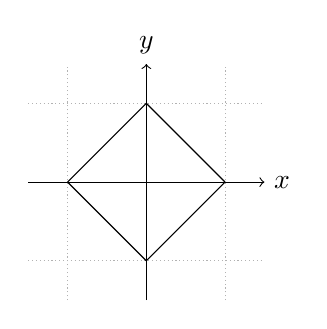
\begin{tikzpicture}
                \draw[style=thin,densely dotted, black!30] (-1.5, -1.5) grid (1.5,1.5);
                \draw[->] (-1.5, 0) -- (1.5,0) node[right] {$x$};
                \draw[->] (0,-1.5) -- (0,1.5) node[above] {$y$};
                \draw (1,0) -- (0,1);
                \draw (0,1) -- (-1,0);
                \draw (-1,0) -- (0,-1);
                \draw (0,-1) -- (1,0);
            \end{tikzpicture}
        \caption{$B_1^1(0,0)$}
        \end{subfigure}

        \begin{subfigure}[c]{.40\textwidth}
            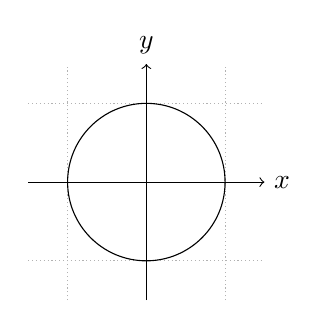
\begin{tikzpicture}
                \draw[style=thin,densely dotted, black!30] (-1.5, -1.5) grid (1.5,1.5);                
                \draw[->] (-1.5, 0) -- (1.5,0) node[right] {$x$};
                \draw[->] (0,-1.5) -- (0,1.5) node[above] {$y$};
                \draw (0,0) circle (1);                
            \end{tikzpicture} 
            \caption{$B_1^2$(0,0)}
        \end{subfigure}
        \begin{subfigure}[c]{.40\textwidth}
            \begin{tikzpicture}
                \draw[style=thin,densely dotted, black!30] (-1.5, -1.5) grid (1.5,1.5);
                \draw[->] (-1.5, 0) -- (1.5,0) node[right] {$x$};
                \draw[->] (0,-1.5) -- (0,1.5) node[above] {$y$};
                \draw (-1,-1) rectangle (1,1);                
            \end{tikzpicture} 
            \caption{$B_1^\infty$(0,0)}
        \end{subfigure}
        \begin{subfigure}[c]{.40\textwidth}
            \begin{tikzpicture}
                \draw[style=thin,densely dotted, black!30] (-1.5, -1.5) grid (1.5,1.5);
                \draw[->] (-1.5, 0) -- (1.5,0) node[right] {$x$};
                \draw[->] (0,-1.5) -- (0,1.5) node[above] {$y$};
                \draw[dashed] (-1,-1) rectangle (1,1);
                \draw[dashed] (1,0) -- (0,1);
                \draw[dashed] (0,1) -- (-1,0);
                \draw[dashed] (-1,0) -- (0,-1);
                \draw[dashed] (0,-1) -- (1,0);п
                \draw (0,0) circle (1);                 
            \end{tikzpicture} 
            \caption{$B_1^p$(0,0)}
        \end{subfigure}
        \caption{Примеры единичных шаров в $l_2^p$}
    \end{figure}
    
    \section{Неполное нормированное пространство}
    \begin{definition}[Финитное линейное пространство]
        \[F = \{ x - \{x_j\}_{j=1}^\infty, x_j \in \bR (\bC) \exists \, N(x) \in \bN : n > N(x) \Rightarrow x_n = 0 \} \]
    \end{definition}
$F \subset l^p \quad 1 \leq p \leq + \infty$.
$(F, || \cdot ||_p) $~--- не полное, $F$~--- не замкнуто.
Будем брать геометрическую прогрессию и обрывать ее на некотором члене.
\begin{gather*}
    x^{(m)} = \left\{ \frac{1}{2}, \frac{1}{4}, \ldots, \frac{1}{2^m}, 0, 0, 0, \ldots \right\} \in F \\
    x = \left\{ \frac{1}{2^k}\right\}^\infty_{k=1} \in l^p \\
    1 \leq p < + \infty \quad ||x - x^{(m)}||_p = \left( \sum^\infty_{k=m+1} \frac{1}{2^{kp}} \right)^{\frac{1}{p}} \underset{m \to \infty}{\longrightarrow} 0
\end{gather*}
Следовательно, $F$~--- не замкнуто.

В качестве упражнения проверить, что $\overline{F}$ в $l^p = ? $ при $p < + \infty$ и при $p = \infty$.
\begin{theorem}
    $C[a,b], ||f||_p = \left( \int^b_a |f(x)|^p dx \right)^{\frac{1}{p}}, 1 \leq p < + \infty$
    \[ (C[a,b], || \cdot || ) \text {~--- не полное } \]
\end{theorem}
\begin{proof}
    При $p = 1$, $[a,b] = [-1,1], f \in C[a,b], \int^b_a |f(x)|^p dx = 0 \Leftrightarrow f(x) \equiv 0$.
    Предъявим фундаментальную последовательность, предел которой не будет непрерывной функцией.

    $f_n = \begin{cases}
        0 & -1 \leq x \leq 0 \\
        nx & x \in [0, \frac{1}{n}] \\
        1 & x \in [\frac{1}{n}, 1]
    \end{cases}, f \in C[-1,1]$ % тут рисунок f

    $f_n$~--- фундаментальная в $(C[-1,1], p=1)$

    Пусть $ m > n$. %рисунок 2
    \[ \int_{-1}^1 |f_m(x) - f_n(x)| dx = \frac{1}{2} \left( \frac{1}{n} - \frac{1}{m} \right) \leq \frac{1}{2n} \underset{n, m \to \infty}{\longrightarrow} 0 \]

    Пусть $\exists \, f \in C[-1,1] : \normunder{f-f_n}{1} \underset{n \to \infty}{\longrightarrow} 0$ 
    \begin{gather*}
        m \geq n \quad \int^1_{\frac{1}{n}} \underbrace{|f(x) - 1|}_{=0} dx  \underset{m \to \infty}{\longrightarrow} 0  \\
        \text{потому что }\int^1_{\frac{1}{n}} {|f(x) - 1|} dx \leq \int^1_0 |f(x) - f_m(x)|dx \underset{m \to \infty}{\longrightarrow} 0
    \end{gather*}
    $\Rightarrow f(x) = 1, x \in \left[ \frac{1}{n}, 1 \right] \forall n $\\
    \[ \begin{cases}
       \Rightarrow f(x) = 1, x \in (0,1], f \text{ непрерывна }, f(0) = 1\\
        \text{аналогично } f(x) \equiv 0 \text{ на } [-1,0]
    \end{cases} \Rightarrow \text{ противоречие } \]
\end{proof}
\begin{figure}
    \begin{subfigure}{0.40\textwidth}
        \includegraphics*{images/chapter3/incompleteness_cab_1.pdf}
    \end{subfigure}
    \begin{subfigure}{0.40\textwidth}
        \includegraphics*{images/chapter3/incompleteness_cab_2.pdf}
    \end{subfigure}
    \caption{Доказательство теоремы 3.7}
\end{figure}

\section{Пополнение метрического пространства}

Мы привели несколько примеров нормированных пространств, не являющихся полными. Приведём еще один пример.
\begin{definition}
    \[ \Rho = \left\{ p(x) = \sum^n_{k=0}a_k x^k, a_k \in \bR, n \geq 0 \right\} \]
\end{definition}
$\Rho$ (подпространство в алгебраическом смысле) $ \subset C[a,b], \, ||p||_\infty = \max_{x \in [a,b]} |p(x)|$

$e^x \notin \Rho$, $p_n(x) = \sum^n_{k=0} \frac{x^k}{k!}, \Rightarrow p_n \darrow{[a,b], n \to \infty} e^x$
это не многочлен, потому что если сколько-то раз продифференцировать многочлен, он станет тождественным 0.

$\Rightarrow \overline{\Rho} \setminus \Rho \ni e^x \Rightarrow \Rho$~--- не замкнуто $\Rightarrow \Rho$~--- не полное.

\[ \overline{\Rho} = C[a,b] \]
\begin{theorem}[Вейерштрасса, 1885]
    $f \in C[a,b], \forall \varepsilon > 0 \, \exists p \in \Rho$ т.ч.  $||f - p|| < \varepsilon$
    (любую функцию на отрезке можно приблизить многочленами)
\end{theorem}

% тту рисунок отрезок в области G открытой, какую бы пилу не нарисовали, ее можно приблизить многочленами$
\[ p_n \darrow{G} f \Rightarrow f \text{ аналитическая в } G \]

Несколько простых свойств метрики, и все следуют из неравенства треугольника
\begin{theorem}[Свойства метрики]
    \label{chap3:metric-props}
    $(X, \rho)$~--- метрическое
    \begin{enumerate}
        \item $x,y,z,u \in X \quad \Rightarrow |\rho(x, u) - \rho(y, z)| \leq \rho(x,y) + \rho(u,z)$
        \item $\rho: X \times X \rightarrow \bR \Rightarrow \rho(x,y)$~--- непрерывная функция
        \item $A \subset X, A $~--- подмножество, $\rho(x,A) = \inf_{y \in A} \rho(x,y) \Rightarrow \rho(x,A)$~--- непрерывная функция от $x$
        \item $A \subset X, A = \overline{A}, x_0 \notin A \Rightarrow \rho(x_0, A) > 0 $
    \end{enumerate}
    
\end{theorem}
\begin{proof}
    \begin{enumerate}
        \item $\rho(x,u) \leq \rho(x,y) + \rho(y,u) \leq \rho(x,y) + \rho(y,z) + \rho(z,u) \Rightarrow \rho(x,u) - \rho(y,z) \leq \rho(x,y) + \rho(z,u)$
        Аналогично $\rho(y,z) - \rho(x,u) \leq \ldots$
        из всего $\Rightarrow 1)$
        \item Докажем непрерывность с помощью последовательности. \\
         $\rho(x,y)$~--- непрерывная?
         \[ \liml_{n \to \infty} x_n = x, \liml_{n \to \infty} y_n = y \Leftrightarrow \liml_{n \to \infty} \rho(x_n, x) = 0 = \liml_{n \to \infty} \rho(y_n, y) \]
         $\rho(x,y) - \rho(x_n, y_n)| \stackrel{(1)}{\leq} \rho(x, x_n) + \rho(y, y_n) \underset{n \to \infty}{\longrightarrow} 0 \Rightarrow \liml_{n \to \infty} \rho(x_n, y_n) = \rho(x,y)$
         \item $A \subset X, \, x,z \in X, \, |\rho(x,A) - \rho(z,A)| \leq ? $ \\
         Пусть $y \in A$
         \begin{multline*}
            \rho(x,y) \leq \rho(x,z) + \rho(z,y) \Rightarrow \rho(x,A) \leq \rho(x,z) + \rho(z,y) \, \forall y \in A \\
            \Rightarrow \rho(x,A) \leq \rho(x,z) + \inf_{y \in A} \rho(z,y) = \rho(x,z) + \rho(z,A) \Rightarrow \\
            \rho(x,A) - \rho(z,A) \leq \rho(x,z)
         \end{multline*}
         Но нам нужен модуль. Можем сказать, что $x$ и $z$ ничем не отличаются, аналогично $\rho(z,A) - \rho(x,A) \leq \rho(x,z) \Rightarrow 3 $
         \item  \[ x_0 \notin A \Rightarrow x_0 \in X \setminus A \text{ открытое} \]
         $\Rightarrow \exists \delta > 0 \quad B_\delta(x_0) \subset X \setminus A \Rightarrow \rho(x_0, A) \geq \delta$
    \end{enumerate}

\end{proof}
Перед определением пополнения нам потребуется несколько определений, связанных с отображениями в метрических пространствах.

$(X, \rho), (Y, d)$~--- метрические пространства. $T: X \rightarrow Y$.
\begin{definition}[Изометрическое вложение]
    \[ d(T_x, T_z) = \rho(x,z) \quad \forall x,z \in X \]
Обозначение: $ X \hookrightarrow Y$
\end{definition}

\begin{definition}[Изометрия]
    $T$~--- изометрическое вложение, $T(X) = Y$
    
\end{definition}
\begin{definition}[Изометричность пространств]
    $(X, \rho), (Y,d)$ изометричны, если $\exists T: X \rightarrow Y, T$~--- изометрия
\end{definition}

\begin{property}
    $T$~--- изометрическое вложение $\Rightarrow$ $T$~--- инъективное, непрерывное
\end{property}
\begin{proof} 
    $x, z \in X, T: X \rightarrow Y,$ пусть $T_x = T_z \Rightarrow d(T_x, T_z) = 0$ 
    Значит, исходное расстояние тоже 0 по свойству метрики. $d(x,z) = 0 \Rightarrow x = z$

    Инъективность проверили, теперь непрерывность, это еще проще.
    \[ \liml_{n \to \infty} x_n = x \Leftrightarrow \liml_{n \to \infty} \rho(x, x_n) = 0 \Rightarrow \liml_{n \to \infty} d(T_{x_n}, T_x) = 0 \Rightarrow \liml_{n \to \infty} T_{x_n} = T_x \]

\end{proof}

\begin{property}
    Если $T$~--- изометрия, то $\exists T^{-1}$~--- изометрия.
\end{property}

\begin{property}
    <<Изометричность>>~--- отношение эквивалентности на множестве метрических пространств
\end{property}

И наконец

\begin{definition}[Пополнение м. пространства]
    $(X, \rho)$~--- метрическое пространство. $(Z, d)$~--- полное метрическое пространство.
    $(Z,d)$~--- пополнение $(X, \rho)$, если существует $T: X \rightarrow Z$
    \begin{enumerate}
        \item $T$~--- изометрическое вложение
        \item $\overline{T(X)} = Z$
    \end{enumerate}
\end{definition}

\begin{remark}
    Не обязательно искать пространство, удовлетворяющее и второму свойству. Достаточно найти такое, которое удовлетворяет первому.
    $(X,\rho)$~--- метрическое пространство, $(U,d)$~--- полное метрическое пространство. Пусть $\exists T: X \rightarrow U$~--- изометрическое вложение. Если 2 свойство не выполняется, то легко такое $Z$ построить.
     Возьмём замыкание образа.
     $ Z = \overline{T(X)} \Rightarrow (Z,d)$~--- пополнение X.
\end{remark}
Теперь обещанная теорема. Возьмём любое метрическое пространство и покажем, что у него есть пополнение.
\begin{theorem}[О пополнении метрического пространства]
    $(X, \rho)$~--- метрическое $\Rightarrow \, \exists$ пополнение $(Z,d)$
\end{theorem}

\begin{proof}
    Есть классическое доказательство с рассмотрением всех фундаметнальных последовательностей, рассмотрением фактор-пространства, 
    муторным разбором случаев. Мы пойдем другим путём. 
    Будет короткое, но \textbf{фантастически}
    непонятное доказательство в том смысле, что непонятно, как его придумать. \\
    Мы собираемся использовать $m(X) = \{ f: X \rightarrow \bR, \sup_{x \in X} |f(x)| < + \infty \} $
    \[ ||f||_{m(X)} = ||f||_\infty = \sup_{x \in X} |f(x)| \]
    $m(X)$~--- полное пространство. \\
    Каждой точке мы сопоставим функцию. Вот такая идея!
    $\varphi: X \rightarrow m(X)$.
    Оно же будет изометрическим вложением, то есть будет сохранять расстояния.  \\
    Сначала будет маленькое облегчающее предположение про $X$, от которого мы потом откажемся.
    Пусть $X$~--- ограниченное, то есть $\exists \, M > 0$ т.ч. $\forall x,y \in X \, \rho(x,y) \leq M$.
    Единственная цель предположения~--- формула для $\varphi$ будет чуть проще. Вообще, можно было бы обойтись и без него. \\
    $t \in X, t$~--- фиксирован, $f_t(x) = \rho(x,t)$.
    При фиксированном $t$~--- это функция на $X$. Именно сюда наше отображение будет отображать $t$. Одной точке~--- целая функция, понятно?

    \[ \varphi(t) := f_t(x) \text{ т.е. } \varphi: t \mapsto f_t(x) \]
    \[ |f_t(x)| \leq M \Rightarrow f_t \in m(X) \]
    Самое главное. Проверим, что отображение сохраняет расстояния. Это очень легко. Возьмём 2 точки.
    \begin{gather*}
        \text{ Пусть } t, s \in X, \quad ||f_t - f_s||_\infty = \sup_{x \in X} |\rho(x,t) - \rho(x,s)|\\
        |\rho(x,t) - \rho(x,s) | \leq \rho(t,s), \, \text { Пусть } x = t \Rightarrow |\rho(t,t) - \rho(t,s) | = \rho(t,s)
    \end{gather*}
    то есть супремум достигается. Естественно, с таким же успехом можно было взять $x = s$
    \[ \Rightarrow  || \varphi(t) - \varphi(s)||_\infty = \rho(t,s) \Rightarrow \varphi \text{~--- изометрическое вложение} \]

    Посмотрим, что будет, если откажемся от этого облегчающего предположения. Надо будет чуть исправить отображение $\varphi$.
    $X$~--- любое метрическое пространство. $a \in X$~--- фиксированная точка.\\
    $t \in X, f_t(x) = \rho(x,t) - \rho(x,a) \Rightarrow |f_t(x)| \leq \rho(a,t) \Rightarrow f_t \in m(X) $

    Раньше мы могли так брать и не вылетать из пространства из-за ограниченности. Вычтем эту штуку, чтобы попасть, куда надо. \\
    \[ t,s \in X \Rightarrow f_t(x) - f_s(x) = \rho(x,t) - \rho(x,s) \stackrel{(1)}{\Rightarrow} 
        ||f_t - f_s||_\infty = \rho(s,t) 
        \]
    Пополнение $X$: $ \overline{\varphi(X)}^{|| \cdot ||_\infty} = Z, (Z, || \cdot ||_\infty) $
\end{proof}

Таким образом, изучение метрических пространств можно свести к изучению подмножества пространства непрерывных функций.
\begin{remark}
    Забегая далеко вперёд.
    $(X, || \cdot ||)$~--- нормированное, $X^*$~--- множество непрерывных линейных функционалов на $X$, $X^*$~--- полное (ВСЕГДА).

    Мы построим каноническое вложение $\pi: X \rightarrow \underbrace{(X^*)^*}_{\text{полное}}$,
    $\overline{\varphi(x)}^{X^{**}}$~--- пополнение X.
\end{remark}


\section{Теорема о вложенных шарах}

Когда-то в анализе была теорема Кантора о том, что если есть последовательность вложенных друг в друга отрезков, то их пересечение не пусто. Мы докажем похожее утверждение для метрических пространств. Оказывается, то утверждение
было связано с полнотой вещественной прямой $\bR$.
$(X, \rho)$~--- метрическое пространство, $r > 0, x \in X$ \\
Введём стандартное обозначение замкнутого шара. 

\[ D_r(x) = \{ y \in X: \rho(x,y) \leq r\}\]

\begin{theorem}[О вложенных шарах]
    $(X, \rho)$~--- метрическое пространство. $X$~--- полное $\Leftrightarrow (\forall \{D_n \}^\infty_{n=1}, D_n = D_{r_n}(x_n)$, $D_{n+1} \subset D_n, 
    \liml_{n \to \infty} r_n = 0 \Rightarrow \bigcap^{+\infty}_{n=1} D_n \neq \varnothing$).
\end{theorem}
По сранению с теоремой Кантора у нас есть дополнительное предположение о стремлении к нулю, которое здесь важно, а на прямой было как данность.

\begin{proof}
    $\Rightarrow \quad X$~--- полное  \\
    \[ \{D_n\}^\infty_{n=1}, D_n = D_{r_n}(x_n), D_{n+1} \subset D_n, \liml_{n \to \infty} r_n = 0  \]
    Надо проверить, что центры шаров образуют фундаментальную последовательность, то есть что $\seq{x_n}^\infty_{n=1}$~--- фундаментальная. \\
    Пусть $\varepsilon > 0 \quad \exists \, N \in \bN \quad r_n < \varepsilon$ при $n \geq N$.
    \begin{multline*}
        (n > N \, \wedge \, m > N) \Rightarrow (x_n \in D_n \, \wedge \, x_m \in D_n) \Rightarrow \rho(x_n, x_m) \leq  \\ 
        \leq \rho(x_n, x_N) + \rho(x_m, x_N) \leq 2 \varepsilon
    \end{multline*}
    \begin{gather*}
        X \text{~--- полное } \Rightarrow \exists \liml_{n \to \infty} x_n = x \\
        \text{ любое фиксированное } m \in \bN \quad x_n \in D_m \, \forall n \geq m, D_m \text{~--- замкнутое } \\
        \Rightarrow \liml_{n \to \infty, n \geq m} x_n = x \in D_m \\
        \Rightarrow x \in \bigcap^\infty_{m=1} D_m
    \end{gather*}
    $\Leftarrow$ \\
    Ничего кроме определения для доказательства полноты у нас нет. Пусть $\seq{x_n}^\infty_{n=1}$~--- фундаментальная.
    Возьмём достаточно быстро убывающую последовательность $\varepsilon_k = \frac{1}{2^k}$. Существует $\seq{x_{n_k}}^\infty_{k=1}, \rho(x_{n_k}, x_{n_{k+1}}) < \frac{1}{2^{k+1}}$. \\
    $D_k = D_{\varepsilon_k} (x_{n_k})$
    
    \begin{figure}
        \centering
        \includegraphics*[width=0.2\textwidth]{images/chapter3/nested_balls_theorem.pdf}
    \end{figure}

    \begin{gather*}
        \begin{cases}
            y \in D_{k+1} \Rightarrow \rho(y, x_{n_{k+1}}) \leq \frac{1}{2^{k+1}} \\
            \rho(x_{n_k}, x_{n_{k+1}}) < \frac{1}{2^{k+1}}
        \end{cases} \Rightarrow 
    \end{gather*}
    \begin{multline*}
        \rho(y, x_{n_k}) \leq \rho(y, x_{n_{k+1}}) + \rho(x_{n_{k+1}}, x_{n_k}) < \frac{1}{2^{k+1}} + \frac{1}{2^{k+1}} = \frac{1}{2^k} \\
        \Rightarrow y \in D_k \Rightarrow D_{k+1} \subset D_k
    \end{multline*}
    Мы взяли произвольный элемент из $D_{k+1}$ и показали, что он принадлежит $D_k$, то есть показали вложенность элементов последовательности.

    \[ \Rightarrow \exists x \in \bigcap^\infty_{k=1} D_k \quad \rho(x, x_{n_k}) \leq \frac{1}{2^k} \Rightarrow \liml_{k \to \infty} x_{n_k} = x \]

    По свойству фундаментальных последовательностей из первой лекции $\liml_{n \to \infty} x_n = x$
\end{proof}

\begin{remark}
    В условиях теоремы пересечение вложенных шаров $\bigcap^\infty_{n=1} D_n$ состоит из одной точки.
\end{remark}

\begin{proof}
    Пусть $x \in \bigcap^\infty_{n=1} D_n, \Rightarrow \rho(x, x_n) < r_n, \liml_{n \to \infty} r_n = 0 \Rightarrow \liml_{n \to \infty} x_n = x$.
    А мы знаем, что предел в метрическом пространстве единственный.
\end{proof}

\begin{remark}
    Условие, что $\liml_{n \to \infty} r_n = 0$ в теореме существенно.
\end{remark}

\begin{example}[Замкнутые множества]
    $\{ F_n \}^\infty_{n=1}, F_n$~--- замкнутое, $F_{n+1} \subset F_n, F_n \subset \bR, \bigcap^\infty_{n=1} F_n = \varnothing, F_n = [n, + \infty)$
\end{example}


\begin{example}[По теореме]
    \[ X =  [1, +\infty) \quad \rho(x,y) = \begin{cases}
        1 + \frac{1}{x+y}, \quad x \ne y \\
        0, \quad x = y
    \end{cases} \]
    Проверим, что $\rho$~--- метрика. $x,y,z$
    \[ \rho(x,y) + \rho(y,z) = 1 + \frac{1}{x+y} + 1 + \frac{1}{y+z} > 1 + 1 > 1 + \frac{1}{x+z} = \rho(x,z) \]
    Проверяем полноту. Пусть $\seq{x_n}^\infty_{n=1}$ фундаментальная, $\varepsilon = \frac{1}{2} \Rightarrow$ 
    \begin{gather*}
        \exists \, N \in \bN : (n \geq N \, \wedge \, m \geq N) \rho(x_n, x_m) < \frac{1}{2} \Rightarrow \left(\rho(x_n, x_N) < \frac{1}{2} \, \wedge \, \rho(x_m, x_N) < \frac{1}{2}\right) \Rightarrow \\
        x_N = x_{N+1} = x_{N+2} = \ldots \\
        \Rightarrow  \, \exists \liml_{n \to \infty} x_n = X_N \Rightarrow (X, \rho) \text{~--- полное}
    \end{gather*}
    Полноту проверили. \\
    $r_n = 1 + \frac{1}{2n}, x_n = n; D_n = D_{r_n}(n), n \in D_n$. Пусть $x \ne n, x \in D_n \Rightarrow \rho(x, x_n) = 1 + \frac{1}{x+n} \leq 1 + \frac{1}{2n}$
\end{example}

\begin{remark}[Домашнее задание]
    Если $(X, || \cdot ||)$~--- банахово, то $\{ D_n \}^\infty_{n=1}, D_{n+1} \subset D_n \Rightarrow \bigcap^\infty_{n=1} D_n \ne \varnothing$  (требование $\liml_{n \to \infty} r_n = 0$ лишнее)
\end{remark}

\section{Сепарабельные пространства}

$(X, \rho)$~--- метрическое пространство,
\begin{definition}[$A$ плотно в $C$]
     $A \subset X, C \subset X$. $A$ плотно в $C$, если $C \subset \overline{A} \Leftrightarrow$
    \[ \forall x \in C \, \forall \varepsilon > 0 \, \exists a \in A \, \rho(x,a) < \varepsilon \Leftrightarrow \forall \varepsilon > 0 \, C \subset \bigcup_{a \in A} B_{\varepsilon}(a) \]
\end{definition}

Любой элемент $C$ можно сколь угодно хорошо приблизить элементами из $A$.

\begin{definition}[$A$ всюду плотно в $X$]
    $A$~--- всюду плотно в $X$, если $\overline{A} = X$
\end{definition}

Чем же полезно это свойство? Если хотят доказать свойство для $X$, то часто доказывают сначала для всюду плотного 
подмножества.

\begin{definition}[Сепарабельное пространство]
    $(X, \rho)$~--- \textbf{сепарабельное}, если $\, \exists E \subset X, E = \seq{x_n}_{n=1}^\infty, \overline{E} = X$
\end{definition}

\begin{theorem}
    $n \in \bN, 1 \leq p \leq +\infty$, 
    \[l^p_n \text{~--- сепарабельное} \]
\end{theorem}

\begin{proof}
    \begin{gather*}
        l^p_n = ( \bR^n, || \cdot ||_p) = \{ x = (x_1, \ldots, x_n), x_j \in \bR, ||x||_p \} \\
        E = \bQ^n = \{ x = (x_1, \ldots, x_n), x_j \in \bQ \}
    \end{gather*}
    Если $ (\bC^n, || \cdot ||_p), \tilde{\bQ} = \{ x + iy, \, x, y \in \bQ \}, E = \tilde{\bQ}^n$
\end{proof}

Знаем, что сходимость в $l^p_n$ эквивалентна покоординатной сходимости, так что если что-то сходится в $\bR$, а $\bQ$ всюду плотно в $\bR$, то $\bQ^n$ всюду плотно в $\bR^n$
\begin{theorem}
    $F$~--- финитные последовательности, $1 \leq p \leq +\infty$
    \[ (F, || \cdot ||_p) \text{~--- сепарабельно} \]
\end{theorem}
\begin{proof}
    $(F, \norm{\cdot}_p) = \bigcup^\infty_{n=1} l^p_n$ (если мы дополним нулями $x$) Тогда $E = \bigcup^\infty_{n=1} \bQ^n = \{ x = (x_1, x_2, \ldots, x_{N(x)}, 0, 0, \ldots, ), x_j \in \bQ \}$.
    Попросту говоря, все финитные последовательности, координаты которых рациональны.
\end{proof}

\begin{theorem}
    $l^p, 1 \leq p < + \infty, c_0$~--- сепарабельные
\end{theorem}
\begin{proof}
    На прошлой лекции мы доказали, что 
    \begin{gather*}
        (F, ||\cdot||_p), \overline{F}^{||\cdot||_p} \text{ (замыкание по норме) } = l^p \text{ при } 1 \leq p < + \infty \\
        \begin{cases}
             E = \bigcup^\infty_{n=1} \bQ^n \text{~--- всюду плотное в } F \\
             F \text{~--- всюду плотное в } l^p \end{cases} \Rightarrow  \\
             E \text{ всюду плотно в } l^p, 1 \leq p < + \infty 
    \end{gather*}
    Почему любой элемент из $l^p$ может быть приближен финитной последоватностью? Мы ее просто отрезаем (\textit{как я понимаю, когда у финитной последовательности набирается норма, достаточно близкая к норме элемента} $l^p$).
\end{proof}

Ответ на упражнение для читателя, которое было на прошлой лекции: 
$F$~--- подпространство в алгебраическом смысле, $F \subset l^\infty$, $\overline{F}^{|| \cdot ||_\infty} = c_0$
\begin{gather*}
    x_0 \in c_0 \Leftrightarrow x = \seq{x_n}^\infty_{n=1}, \liml_{n \to \infty} x_n = 0 \\
    \text{ берем первые } m \text { координат и дополняем их нулями } \\
    x^{(m)} = (x_1, \ldots, x_m, 0, 0, \ldots, 0, \ldots) \Rightarrow x^{(m)} \in F \\
    ||x - x^{(m)}||_\infty = \sup_{k > m} |x_k| \underset{m \to \infty}{\longrightarrow} 0
\end{gather*}
Любой элемент из $c_0$ является пределом последовательности элементов из $F$ по норме $\norm{\cdot}_\infty$.


Остаётся вопрос, почему $c_0$~--- замкнутое множество. Можно в лоб, а можно по-учёному рассудить.
\begin{gather*}
    \text{ пусть } \seq{y^{(m)}}^\infty_{m=1}, y^{(m)} \in c_0, \, y^{(m)} \underset{m \to \infty}{\longrightarrow} y \text{ в } c_0 \\
    \Rightarrow \liml_{m \to \infty} ||y - y^{(m)}||_\infty = 0 \qquad y = \{ y_n \}^\infty_{n=1}, \text{ хотим доказать }\liml_{n \to \infty} y_n = 0
\end{gather*}
А это равномерная сходимость на множестве натуральных чисел. Здесь $y$  и $y_m$ --- непрерывные функции на множестве натуральных чисел. То есть это тот случай, когда можно менять местами пределы (были такие умные 
теоремы в анализе)
\[ \liml_{n \to \infty} y_n = \liml_{m \to \infty} \underbrace{\liml_{n \to \infty} y_n^{(m)}}_{=0} = 0 \]

Упражнение: $c$~--- сепарабельное, $c \subset l^\infty$ 

\begin{theorem}
    $l^\infty$~--- не сепарабельное
\end{theorem}

Всюду плотное $\Leftrightarrow$ какой бы шарик из $X$ мы бы не предъявили, там всегда будет элемент всюду плотного множества. Как доказывать несепарабельность?
Построим гигантское, несчётное число непересекающихся шариков. И скажем, что если какое-то множество --- всюду плотное, то в каждом из них должен быть представитель, а шарики-то не пересекаются, значит в каждом должен быть
свой представитель. Значит, счётного всюду плотного --- нет.

\begin{proof}
    Рассмотрим специальные последовательности, состоящие только из нулей и единиц. Рассмотрим последовательность, являющуюся в точности характеристической функцией $A$
    \[
        A \subset \bN \quad x^A_n = \begin{cases}
            1 & n \in A \\
            0 & n \notin A
        \end{cases}\]
    Для каждого набора натуральных чисел рассмотрим вот такую последовательность. Когда координата принадлежит множеству $A$, будет 1, иначе --- 0. Например, 
    $A = \{ 2, 3 \}$, $x^A_n = \{ 0, 1, 1, 0, 0, \ldots \}$.

    Мощность $\{A, A \subset \bN \}$~--- континуум (> счётное). Это и будут центры наших пересекающихся шариков. Посмотрим, каким будет расстояние между двумя разными точками.
    \begin{gather*}
        A \subset \bN, C \subset \bN, A \ne C \\
        x^A_n - x^C_n = \begin{cases}
            1 \\
            0 \\
            -1
        \end{cases} 
        \intertext{всех нулей не бывает, поскольку множества не совпадают}
        \Rightarrow ||x^A - x^C||_\infty = \sup_{n \in \bN} |x^A_n - x^C_n| = 1 
    \end{gather*}
    То есть если 2 множества не равны, то расстояние между ними~--- единица.

    \[B_{\frac{1}{2}} (x^A) \cap B_{\frac{1}{2}}(x^C) = \varnothing \] 
    Мы предъявили несчётный набор дизъюнктных шариков. Пусть $E$~--- всюду плотно в $l^\infty \Rightarrow \, \forall A \subset \bN \, \exists e_A \in B_{\frac{1}{2}}(x^A)$

    \[ A \ne C \Rightarrow e_A \ne e_C, \qquad \underbrace{\seq{e_A}_{A \subset \bN}}_{\text{ несчётно }} \subset E \Rightarrow E \text{ несчётно } \]
    На пальцах: $x^A \in l^\infty$. Если есть какое-то всюду плотное множество, то его элемент должен лежать в любой окрестности (пусть $\varepsilon = \frac{1}{2}$) $x^A$. Все $x^A$ для $\forall A \subset N$ отделены друг от друга единицей. Это значит, что $x^A, x^C, A \ne C$ не может обслуживать
    один $e_I$. Иначе $\rho(x^A, x^C) \leq \rho(x^A, e_A) + \rho(x^C, e_C) < 1$. То есть для каждого $x^A$ он свой, а их несчётное количество.  
\end{proof}
То, что у всех шариков одинаковый радиус~--- это просто приятный бонус.

\begin{theorem}
    $(X, \rho)$~--- сепарабельное, $ Y \subset X \Rightarrow (Y, \rho)$~--- сепарабельное. 
\end{theorem}
\begin{proof}
    $\exists \, E = \seq{x_n}^\infty_{n=1}$~--- всюду плотно в $X$, $x_0 \in X$
    \begin{gather*}
    \rho(x_n, Y) = \inf_{y \in Y} \rho(x_n, y) \Rightarrow \\
    \exists \, \seq{y_{n,k}}^\infty_{k=1} \quad \liml_{k \to \infty} \rho(x_n, y_{n,k}) = \rho(x_n, Y) \\ 
    y_{n,k} \in Y, \, F = \seq{y_{n_k}}_{n,k} \text{~--- счётное }, F \subset Y    
    \end{gather*}
    Проверим, что $F$~--- всюду плотно в $Y$. Пусть $y \in Y, \varepsilon > 0 \Rightarrow \, \exists x_n : \rho(y, x_n) < \varepsilon$.
    Из этого неравенства мы делаем вывод, что $\rho(x_n, Y) < \varepsilon$. Значит, $\exists k: \rho(x_n, y_{n,k}) < \varepsilon \Rightarrow$
    \[ \rho(y, y_{n,k}) \leq \rho(y, x_n) + \rho(x_n, y_{n,k}) < \varepsilon + \varepsilon = 2 \varepsilon \]
\end{proof}

\begin{corollary}
    $X$~--- бесконечное множество $\Rightarrow m(X) $~--- не сепарабельное.  
\end{corollary}
\begin{proof}
    Можно слово в слово повторить доказательство для $l^\infty$, но мы воспользуемся последними доказанными теоремами.
    \begin{gather*}
        \exists \seq{a_j}^\infty_{j=1}, a_j \in X, a_j \ne a_i \text{ при } i \ne j \\
        Y = \{ f \in m(X), f(x) = 0 \text{ если } x \ne a_j \} \sup_{j \in \bN} |f(a_j)| < + \infty \\
        Y \text{ изометрично } l^\infty, f \in Y, T(f) = \seq{f(a_j)}^\infty_{j=1} \in l^\infty \\
        Y \text{~--- не сепарабельно } \Rightarrow \text{ и по последней теореме } \\
        m(X) \text{~--- не сепарабельно}
    \end{gather*}
\end{proof}

\begin{theorem}
    \[ C[a,b] \text {~--- сепарабельно} \]
\end{theorem}
\begin{proof}[1 часть]
    \begin{gather*}
        L = \{ \text{ ломаные } \} \quad a = x_0 < x_1 < \ldots < x_n = b \quad \seq{y_k}^n_{k=0}, y_k \in \bR \\
        L(x) \text{~--- ломаные} \\
        L(x_k) = y_k, \, k = 0,1, \ldots, n \quad l(x) \text{ линейная на } [x_k, x_{k+1}]
    \end{gather*}
    Отметим, что $L$~--- всюду плотное множество в пространстве непрерывных функций. Это связано с равномерной непрерывностью. 
    Никаких надежд на то, что оно будёт счётным нет.
    \begin{gather*}
        \text{ пусть } f \in C[a,b], \, \varepsilon > 0 \Rightarrow \exists \delta > 0 : |x-y| < \delta \\
        \Rightarrow |f(x) - f(y)| < \varepsilon \\
        \exists \seq{x_k}^n_{k=0} \text{~--- разбиение } \quad x_{k+1} - x_k < \delta \\
        y_k := f(x_k) \quad L(x) \text{~--- ломаная } \\
        \Rightarrow |f(x) - L(x)| < \varepsilon \Rightarrow ||f-L||_\infty \leq \varepsilon \Rightarrow \overline{\calL} = C[a,b] \\
    \end{gather*}
    как сделать так, чтобы множество ломаных было счётным? возьмём в качестве вершин элементы $\bQ$
    \begin{gather*}
        E = \{ L \in \calL, \, x_k, y_k \in \bQ \} \text{~--- счетное множество } \\
        \begin{cases}
            \calL \subset \overline{E} \\
            \overline{\calL} = C[a,b]
        \end{cases} \Rightarrow E \text{~--- всюду плотно, т.е. } \overline{E} = C[a,b]
    \end{gather*}
    
\end{proof}

\begin{proof}[2 часть]
    по т. Вейерштрасса замыкание многочленов~--- тоже пространство непрерывных функций.
    \begin{gather*}
        \Rho = \{ p(x) = \sum^n_{k=0} a_k x^k \} \quad \overline{\Rho} = C[a,b] \\
        E = \{ p(x) = \sum^n_{k=0} a_k x^k, \, a_k \in \bQ \} \\
        \begin{cases}
            \Rho \subset \overline{E} \\
            \overline{\Rho} = C[a,b]
        \end{cases} \Rightarrow \overline{E} = C[a,b]
    \end{gather*}
\end{proof}


\section{Нигде не плотные множества}

\begin{definition}
    $(X, \rho)$~--- метрическое пространство. $A \subset X, A$~--- \textbf{ нигде не плотно} в $X$, если 
    \[ \forall B_r(x) \text { при } r > 0, x \in X \quad B_r(x) \not \subset \overline{A} \Leftrightarrow \Int(\overline{A}) = \varnothing \Leftrightarrow \]
\end{definition}
Если мы рассмотрим замыкание, никакого шарика там не будет. Иначе: если мы рассмотрим внутренность замыкания, она будет пустой.

\begin{multline*}
    \forall r > 0, x \in X \quad B_r(x) \: \exists B_{r_1}(x_1) \subset B_r(x), B_{r_1}(x_1) \cap A = \varnothing \\
    \Leftrightarrow \forall r > 0, x \in X, D_r(x) \: \exists D_{r_1}(x_1) \subset D_r(X), D_{r_1}(x_1) \cap A = \varnothing
\end{multline*}

Скоро докажем связь между нигде не плотными множествами и полными пространствами.
 Но сперва определение, которое не будет часто встречаться, но сам факт~--- полезный.
\begin{definition}[множество первой категории]
    $M \subset X, (X, \rho)$. $M$~--- \textbf{ множество первой категории}, если 
    \[ M = \bigcup^\infty_{j=1} E_j, E_j \text{ нигде не плотно в } X \]
\end{definition}

$M$~--- \textbf{ множество второй категории}, если $M$ нельзя представить в виде объединения счетного числа нигде не плотных множеств.

\begin{theorem}[Бэр, о категориях]
    \label{chap3:baire}
    $(X, \rho)$~--- полное $\Rightarrow X$~--- множество второй категории.
\end{theorem}

\begin{proof}
    Можно было бы даже от противного. Но мы возьмём семейство $\seq{M_j}^\infty_{j=1}$, $M_j$~--- нигде не плотно в $X$, $\, E = \bigcup^\infty_{j=1} M_j$.
      Мы докажем, 
    что найдётся хоть одна точка, которая принадлежит $X$ и не принадлежит $E$. Это и будет обозначать, что $X$ невозможно представить
    в виде такого объединения.
    \begin{gather*}
        x_0 \in X \quad D_0 = \{ y: \rho(x_0, y) \leq 1\} \\
        M_1 \text{~--- нигде не плотно } \Rightarrow \, \exists D_1 = D_{r_1}(x_1) \subset D_0, D_1 \cap M_1 = \varnothing \\
        r_1 < 1
    \end{gather*}
    Теперь мы то же соображение применим к множеству $M_2$, которое тоже нигде не плотно
    \begin{gather*}
        \exists D_2 = D_{r_2}(x_2) \subset D_1, D_2 \cap M_2 = \varnothing \\
        r_2 < \frac{1}{2}
    \end{gather*}
    и так далее $\begin{cases}
         \seq{D_n}^\infty_{n=1}, D_n = D_{r_n} (x_n), D_{n+1} \subset D_n \\
         D_n \cap M_n = \varnothing, r_n < \frac{1}{n} \end{cases}$ по теореме о вложенных шарах
         $\Rightarrow \, \exists x \in \bigcap^\infty_{n=1}D_n, (x \in D_n \, \wedge \, x \in X \setminus E) \Rightarrow x \notin M_n \, \forall n \Rightarrow x \notin E$
\end{proof}


\section{Полные семейства элементов}

Теперь мы будем понимать полноту в совершенно другом смысле.
Сначала вспомним, что такое линейная оболочка пространства.
\begin{definition}[Линейная оболочка]
    $X$~--- линейное пространство над $\bR (\bC)$. Рассмотрим семейство $\seq{x_\alpha}_{\alpha \in A}$~--- семейство элементов, $x_\alpha \in X$.
    \[ \calL \seq{x_\alpha}_{\alpha \in A}  = \left\{ \sum^n_{k=1} c_k x_{\alpha_k}, c_k \in \bR (\bC), n \in \bN \right\} \]
\end{definition}


\begin{definition}[Полное семейство]
    $(X, || \cdot ||)$, $\seq{x_\alpha}_{\alpha \in A}$~--- \textbf{полное семейство}, если $\overline{\calL \seq{x_\alpha}_{\alpha \in A}} = X$.
    То есть линейная оболочка всюду плотна в $X$.
\end{definition}

\begin{example}
    $C[a,b], \, \seq{x^n}^{+\infty}_{n=0}$~--- полное семейство в $C[a,b]$, так как
    $\Rho = \calL \seq{x^n}^{+\infty}_{n=0}, \, \overline{\Rho} = C[a,b]$
\end{example}

\begin{example}
    $l^p, \, 1 \leq p < + \infty, \, c_0$
    \begin{gather*}
        e_n = (1, 0, 0, \ldots, 0, \underbrace{1}_n, 0, \ldots), \seq{e_n}^\infty_{n=1} \text{~--- полное семейство} \\
        \calL \seq{e_n}^\infty_{n=1} = F \text{~--- финитная последовательность}
    \end{gather*}
\end{example}

Упражнение: $C$~--- что будет полным семейством?

\begin{statement}
    \label{chap3:statement}
    $(X, || \cdot ||)$ - нормированное пространство. В нём существует $\seq{x_n}^\infty_{n=1}$~--- полное семейство 
    \[ X \text{~--- сепарабельное} \]
\end{statement}
\begin{proof}
    Рассмотрим линейную оболочку $L = \calL \seq{x_n}^\infty_{n=1} = \seq{x = \sum^n_{j=1} c_j x_j, c_j \in \bR (\bC)}$. $\overline{L} = X$.
    \begin{gather*}
        E = \left\{ x = \sum^n_{j=1} c_j x_j, c_j \in \bQ \right\} \text{~--- счётное всюду плотное} \\
        (L \subset \overline{E} \, \wedge \, \overline{L} = X) \Rightarrow \overline{E} = X
    \end{gather*}
\end{proof}

\begin{remark}
    $l^\infty, E = \seq{ x = \seq{x_n}^\infty_{n=1}, x_n \in \bQ, \sup_{n \in \bN} |x_n| < + \infty}$.
    $\overline{E} = l^\infty$, $E$~--- не счётное.
\end{remark}
    
\section{Полные и плотные множества в $L^p$}
Сначала небольшое замечание. $(X, U, \mu)$~--- пространство с мерой $e \in U$~--- измеримые множества, 
$\chi_e(x) = \begin{cases}
    1 & x \in E \\
    0 & x \notin E
\end{cases}$~--- характеристическая функция. $\chi \in L^\infty(X, \mu), \, \forall e \in U$
\[ \chi_e \in L^p(X, \mu) \text{ при } 1 \leq p < + \infty \Leftrightarrow \int_X (\chi_e(x))^p d\mu < + \infty \Leftrightarrow \mu e < + \infty \]

\begin{theorem}
    $(X,U, \mu )$~--- пространство с мерой $\Rightarrow$ 
    \begin{gather*}
        \seq{\chi_e}_{e \in U} \text {~--- полное семейство в } L^\infty(X, \mu) \\
        \seq{\chi_e}_{e \in U, \mu e < + \infty} \text{~--- полное семйество в } L^p(X, \mu), 1 \leq p < + \infty 
    \end{gather*}
\end{theorem}

Для доказательства этой теоремы нужно будет вспомнить теорему Лебега из анализа (она у нас уже была).
\begin{theorem}[Лебег]
    $\seq{h_n(x)}^\infty_{n=1}$~--- измеримые, $\varphi(x)$. $\int_X \varphi(x) d \mu < + \infty, |h_n(x)| \leq \varphi(x)$ п.в. на $X$
    \[ h_n(x) \underset{n \to \infty \text{ п.в. по } \mu}{\longrightarrow} h(x) \Rightarrow \liml_{n \to \infty} \int_X h_n(x) d \mu = \int_X h(x) d \mu \]
    
\end{theorem}

\begin{proof}
    Вспомним конструкцию, которая была в математическом анализе. $f$~--- измеримая, $f(x) \geq 0, x \in X$.
    Рассмотрим разбиение множества $X$, а по нему построим соотвествующую простую функцию
    \begin{gather*}
        n \in \bN \quad e_k = \seq{x \in X: \frac{k}{n} \leq f(x) < \frac{k+1}{n}}, k = 0, 1, \ldots, n^2 - 1 \\
        e_{n^2} = \seq{x: f(x) \geq n} \Rightarrow X = \bigcup^{n^2}_{k=0} e_k, e_k \cap e_j = \varnothing (k \ne j)
    \end{gather*}

    Теперь построим измеримые функции, потом они будут простыми.
    \[g_n(x) = \sum^{n^2}_{k=1} \frac{k}{n} \chi_{e_k}(x) \quad 0 \leq g_n(x) \leq f(x), x \in X \]
    $f(x) \leq g_n(x) + \frac{1}{n}, x \in \bigcup^{n^2-1}_{k=0} e_k$ \\

    Теперь все готово, чтобы обсудить случай $L^\infty$. Пусть $f \in L^\infty(X,\mu) \Rightarrow n \geq ||f||_\infty \Rightarrow \mu(e_{n^2}) = 0 $.
    $\Rightarrow |f(x) - g_n(x)| \leq \frac{1}{n}$ для п.в. $x \in X$ \\
    $\Rightarrow ||f-g_n||_\infty \underset{n \to \infty}{\longrightarrow} 0, g_n \in \calL \seq{\chi_e}_{e \in U}$

    $\Rightarrow f \in \overline{\calL \seq{\chi_e}_{e \in U}}$ \\
    Посмотрим теперь, что происходит с конечными $p$. Тут вспоминаем теорему Лебега, она была верна для интеграла Лебега, но верна и для произвольной меры.
    \begin{gather*}
        \begin{cases}
            f(x) \in L^p(X, \mu), 1 \leq p < + \infty \quad |f(x) - g_n(x)|^p \leq |f(x)|^p \\
            g_n(x) \underset{\text{п.в.}}{\longrightarrow} f(x) \quad \Rightarrow |f(x) - g_n(x)|^p \underset{n \to \infty}{\longrightarrow} 0
        \end{cases} \stackrel{\text{Лебег}}{\Rightarrow} \\
        \liml_{n \to \infty} \left( \int_X |f-g_n|^p d \mu \right)^\frac{1}{p} = 0
        \intertext{все, что надо~--- убедиться, что мера конечная. Покажем, что $f \in L^p \Rightarrow \mu e_k < + \infty $}
        f(x) \geq \frac{k}{n}, x \in e_k \Rightarrow \left( \int_X |f|^p d\mu \right)^\frac{1}{p} \geq \left( \int_{e_k} \left( \frac{k}{n} \right)^p d\mu \right)^\frac{1}{p} = \\
        \frac{k}{n} (\mu e_k)^\frac{1}{p} \Rightarrow \mu e_k < + \infty \\
        \Rightarrow f \in \overline{\calL \seq{\chi_e}_{e \in U, \mu e < + \infty}}
    \end{gather*}
    Теперь покажем, что для произвольных $f$ рассуждение тоже верно.  Рассмотрим замыкание линейное оболочки
    \begin{gather*}
        \begin{cases}
            f: X \rightarrow \bR, \Rightarrow f = f_+ - f_-, f_+(x) \geq 0, f_-(x) \geq 0 \\
            f: X \rightarrow \bC \Rightarrow f = u + iv; u, v: X \rightarrow \bR
        \end{cases} \Rightarrow \\
        \forall f \in L^p, f \in \overline{\calL \seq{\chi_e}_{e \in U}} \\
        (p = \infty \, \forall e, p < + \infty, \mu e < + \infty)
    \end{gather*}
\end{proof}

Теперь, зная эту теорему, посмотрим, какое множество будет полным в пространстве $l^\infty$

\begin{corollary}
    $l^\infty, A \subset \bN$, $x^A = \seq{x^A_n}^\infty_{n=1}, x^A_n = \begin{cases}
        1 & n \in A \\
        0 & n \notin A
    \end{cases} \Rightarrow$
    \[ \seq{x^A}_{A \subset \bN} \text{~--- полное семейство в } l^\infty \]
\end{corollary}

\begin{proof}
    $l^\infty = L^\infty(\bN, \mu), \mu(n) = 1 \, \forall n \in \bN \quad \forall A \subset \bN, A $~--- измеримо 
    \[\chi_A = x^A \Rightarrow \seq{x^A}_{A \subset \bN} \text{~--- полное семейство } \] 
\end{proof}


\begin{theorem}
    $(\bR^n, U, \lambda)$, $\lambda$~--- классическая мера Лебега. $U$~--- измеримые по Лебегу множества. 
    \[ \R = \left\{ \Delta = \prod^n_{j=1} [a_j, b_j), a_j < b_j; a_j, b_j \in \bR \right\} \text{~--- множество ячеек} \]
    \[\Rightarrow \seq{\chi_\Delta}_{\Delta \in \R} \text{~--- полное семейство в } L^p(\bR^n, \lambda), 1 \leq p < + \infty \]
\end{theorem}
Достаточно рассмотреть характеристические множества ячеек.

\begin{proof}
    Собираемся приблизить элемент $\chi_e$ линейной комбинацией характеристических функций ячеек. Вспомним определение внешней меры.
    \begin{gather*}
        e \in U, \lambda(e) < + \infty \\
        \lambda(e) = \inf \left\{ \sum^\infty_{k=1} \lambda(\Delta_k), e \subset \bigcup^\infty_{k=1} \Delta_k, \Delta_k \in \R, \Delta_k \cap \Delta_j = \varnothing \right\}
    \end{gather*}
    Сначала просто по определению нижней грани. $\forall \varepsilon > 0 \Rightarrow \, \exists \seq{\Delta_k}^\infty_{k=1}$.
    $\lambda(e) \leq \sum^\infty_{k=1} \lambda(\Delta_k) < \lambda(e) + \varepsilon$. \\
    $e \subset \bigcup^\infty_{k=1} \Delta_k, \Delta_k \in \R, \Delta_k \cap \Delta_j = \varnothing$ при $k \ne j$. \\
    \begin{gather*}
        A = \bigcup^\infty_{k=1} \Delta_k, e \subset A, \lambda(A \setminus e) < \varepsilon \\
        \exists N \in \bN \quad \sum^\infty_{k=N+1} \lambda(\Delta_k) < \varepsilon, B = \bigcup^n_{k=1} \Delta_k \\
        \Rightarrow \lambda(A \setminus B) < \varepsilon 
    \end{gather*}
    \begin{multline*}
        || \chi_e - \chi_B ||_p \leq ||\chi_e - \chi_A||_p + ||\chi_A - \chi_B||_p \leq \\
        \left( \int_{A \setminus e} \mathbb{1} d\mu \right)^{\frac{1}{p}} + \left( \int_{A \setminus B} \mathbb{1} d\mu \right)^{\frac{1}{p}} < \varepsilon^{\frac{1}{p}} + \varepsilon^{\frac{1}{p}} = 2 \varepsilon^{\frac{1}{p}} 
    \end{multline*}

    \begin{gather*}
        \chi_B = \sum^N_{k=1} \chi_{\Delta_k} \in \calL \seq{\chi_\Delta}_{\Delta \in \R} \\
        \begin{cases}
            \overline{\calL \seq{\chi_e}_{e \in U}} = L^p \\
            \chi_e \in \overline{\calL \seq{\chi_\Delta}_{\Delta \in \R}}
        \end{cases} \Rightarrow \overline{\calL \seq{\chi_\Delta}_{\Delta \in \R}} = L^p, 1 \leq p < + \infty
    \end{gather*}

\end{proof}

\begin{corollary}
    $E \subset \bR^n$, $E$~--- измеримые по Лебегу, $1 \leq p < + \infty$ 
    \[ \Rightarrow L^p(E, \lambda) \text{~--- сепарабельные} \]
    ($\lambda$~--- мера лебега)
\end{corollary}

\begin{proof}
    Докажем, что $L^p(\bR^n, \lambda)$~--- сепарабельное.
    \[ \R = \left\{ \Delta = \prod^n_{j=1} [a_j, b_j), a_j < b_j, \, a_j, b_j \in \bR \right\} \text{~--- полные семейства в } L^p \]
    Теперь мы возьмём только такие ячейки, координаты которых рациональны. Пока что можем
    сказать, что это счётное множество.
    \[  R_0= \left\{ \Delta = \prod^n_{j=1} [a_j, b_j), a_j < b_j, \, a_j, b_j \in \bQ \right\} \text{~--- счётное множество} \]

    \begin{gather*}
        \Delta \in \R \quad \text{пусть } \varepsilon > 0 \\
        \Rightarrow \, \exists \Delta_0 \in R_0, \Delta \subset \Delta_0, \lambda(\Delta_0 \setminus \Delta) < \varepsilon \\
        \Rightarrow || \chi_{\Delta_0} - \chi_{\Delta} ||_p = || \chi_{\Delta_0 \setminus \Delta} ||_p = \left( \int_{\Delta_0 \setminus \Delta}\mathbb{1} dx \right)^{\frac{1}{p}} = 
        \left( \lambda (\Delta_0 \setminus \Delta)\right)^{\frac{1}{p}} < \varepsilon^{\frac{1}{p}} \\
        \Rightarrow \, \forall \Delta \in \R \quad \chi_\Delta \in \overline{\calL \seq{\chi_\Delta}_{\Delta \in R_0}}
     \end{gather*}

     $R_0$~--- полное счётное семейство ${\Rightarrow}$ [[утверждение \hyperref[chap3:statement]{3.1}]] $L^p(\bR^n, \lambda)$~--- сепарабельное.
     \begin{gather*}
        E \subset \bR^n, E \text{~--- измеримое }, f \in L^p(E, \lambda) \\
        \text{ пусть } f(x) = 0, x \in \bR^n \setminus E \Rightarrow f \in L^p(\bR^n, \lambda) \\
        \Rightarrow L^p(E, \lambda) \text{~--- подпространство } L^p(\bR^n, \lambda) \Rightarrow L^p(E, \lambda) \text{~--- сепарабельно}
     \end{gather*}
\end{proof}


\begin{definition}
    $(X, U, \mu)$~--- пространство с мерой. $(X, \rho)$~--- метрическое пространство.
    $\mu$ \textbf{~--- борелевская мера}, если $(G$~--- открытое $\Rightarrow G \in U)$
\end{definition}

$\beta$~--- минимальная $\sigma$-алгебра,  содержащая все открытые множества. $\beta$~--- \textbf{борелевские множества}, то есть $\beta \subset U$.

Чем же хороши борелевские меры? Оказывается, они безумно связаны с непрерывными функциями

\begin{remark}
    Пусть $f: X \rightarrow \bR, f$~--- непрерывная $\Rightarrow f^{-1}((c,+\infty)), c \in \bR, (c, +\infty)$~--- открытое в $\bR$.
    Определение непрерывной функции из топологии: прообраз любого открытого множества открыт.
    Так как прообраз $f$ открыт в $X$ $\Rightarrow f$~--- измеримая по $\mu$, если $\mu$~--- борелевская.

\end{remark}

\begin{remark}
    $\lambda$~--- мера Лебега в $\bR^n$, тогда $\lambda$~--- борелевская.
\end{remark}
Еще более специальное определение. Этим свойством мера Лебега тоже обладает.

\begin{definition}[регулярная мера]
    $(X, U, \mu)$, $(X, \rho)$, $\mu$~--- борелевская. $\mu$~--- \textbf{ регулярная мера}, если $\forall e \in U $
    \[ \sup_{\seq{F \subset e, F \text{~--- замкнутое} }} \seq{ \mu(F)} = \mu e = \inf_{\seq{e \subset G, G \text {~--- открытое}}} \mu G \]
\end{definition}

\begin{remark}
    $\lambda$-мера Лебега~--- регулярная.
\end{remark}

На самом деле эти 2 свойства друг из друга следуют, но мы это доказывать не будем.

\begin{theorem}
    $(X, U, \mu)$, $(X, \rho)$, $\mu$~--- регулярная мера $\Rightarrow$  непрерывные функции плотны в
    $L^p(X, \mu), 1 \leq p < + \infty$.
    \[ \overline{C(X) \cap L^p(X,\mu)}^{|| \cdot ||_p} = L^p(X, \mu) \]
\end{theorem}
\begin{proof}
    Мы уже знаем, что полное семейство~--- это семейство характеристических функций всех
    измеримых функций, и мы будем этим изо всех сил пользоваться. Возьмём какую-то характеристическую функцию из множества и ее будем приближать
    непрерывными функциями. \\
    $\seq{ \chi_e}_{e \in U, \mu e < + \infty }$~--- полное семейство. \\
    пусть $ e \in U, \mu e < + \infty, \, \let \varepsilon > 0, \mu$ ~--- регулярная $\Rightarrow 
    \, \exists F \subset e \subset G, F$~--- замкнутое, $G$~--- открытое. $\mu(G \setminus F) < \varepsilon$
    %символическая картинка
    \[ \varphi(x) = \frac{\rho(x, X \setminus G)}{\rho(x, X \setminus G) + \rho(x, F)} \]
    Когда мы попадем в $X \setminus G$, она будет равна нулю.
    Нужно позаботиться о том, чтобы знаменатель не был равен нулю. \\
    $\rho(x,A)$~--- непрерывная функция $\forall A \subset X$ (теорема \ref{chap3:metric-props}). $X \setminus G$~--- замкнутое, $F$~--- замкнутое.
    Если $\rho(x, F) = 0 \Rightarrow x \in F \Rightarrow x \notin X \setminus G \Rightarrow \rho(x, X \setminus G) > 0$ 
    \[ \Rightarrow \rho(x, X \setminus G) + \rho(x, F) > 0 \: \forall x \in X \Rightarrow \varphi \in C(X) \]

    $\varphi(x) = 0, x \in X \setminus G, \varphi(x) = 1, x \in F \quad \forall x \in X \: 0 \leq \varphi(x) \leq 1$

    Понятно, что модуль $\varphi(x)$ совпадает с характеристической функцией множества $e$.
    \begin{gather*}
        |\chi_e(x) - \varphi(x)| \leq 1 \quad \forall x \in X \\
        \chi_e(x) - \varphi(x) = 0 \quad x \in F \text{ или } x \in X \setminus G \\
        \Rightarrow ||\chi_e - \varphi||_p = \left( \int_X |\chi_e(x) - \varphi(x) |^p d\mu \right)^{\frac{1}{p}} = 
        \left( \int_{G \setminus F} |\chi_e(x) - \varphi(x) |^p d \mu \right)^{\frac{1}{p}} \leq \\
        \leq \left( \mu(G \setminus F) \right)^{\frac{1}{p}} < \varepsilon^{\frac{1}{p}} \\
        \Rightarrow \chi_e \in \overline{C(X)}^{|| \cdot||_p}
    \end{gather*}
    Тем самым мы доказали, что $\chi_e(x)$ может быть приближена непрерывными функциями.
    Может быть, стоить отметить, что 
    $\mu G < \mu e + \varepsilon < +\infty \quad \int_X |\varphi(x)|^p d \mu - \int_G |\varphi(x)|^p d \mu < \mu G \Rightarrow
    \varphi \in L^p(X, \mu)$
    
\end{proof}


Раз утверждение верно для любых регулярных мер, то оно верно и для меры Лебега.
\end{document}
